\documentclass[a4paper, 12pt]{article} % тип документа

%%%Библиотеки
    %\usepackage[warn]{mathtext}	
    \usepackage[T2A]{fontenc}   %Кодировка
    \usepackage[utf8]{inputenc} %Кодировка исходного текста
    \usepackage[english, russian]{babel} %Локализация и переносы
    \usepackage{caption}
    \usepackage{gensymb}
    %\usepackage{listings}
    \usepackage{amsmath, amsfonts, amssymb, amsthm, mathtools}
    %\usepackage[warn]{mathtext}
    %\usepackage[mathscr]{eucal}
    %\usepackage{wasysym}
    %\usepackage{graphicx} %Вставка картинок правильная
    %\usepackage{pgfplots}
    \usepackage{indentfirst}
    %\usepackage{float}    %Плавающие картинки
    %\usepackage{wrapfig}  %Обтекание фигур (таблиц, картинок и прочего)
    \usepackage{fancyhdr}  %Загрузим пакет
    %\usepackage{lscape}
    %\usepackage{xcolor}
    %\usepackage[normalem]{ulem}
    
    \usepackage{titlesec}
    \titlelabel{\thetitle.\quad}

    \usepackage{hyperref}

%%%Конец библиотек

%%%Настройка ссылок
    \hypersetup
    {
        colorlinks = true,
        linkcolor  = blue,
        filecolor  = magenta,
        urlcolor   = blue
    }
%%%Конец настройки ссылок


%%%Настройка колонтитулы
    \pagestyle{fancy}
    \fancyhead{}
    \fancyhead[L]{1.3.2}
    \fancyhead[R]{Глаз Роман, группа Б01-007}
    \fancyfoot[C]{\thepage}
%%%конец настройки колонтитулы



\begin{document}
                        %%%%Начало документа%%%%


%%%Начало титульника
\begin{titlepage}

    \newpage
    \begin{center}
        \normalsize Московский физико-технический институт \\(госудраственный университет)
    \end{center}

    \vspace{6em}

    \begin{center}
        \Large Лабораторная работа по общему курсу физики\\Механика
    \end{center}

    \vspace{1em}

    \begin{center}
        \Large \textbf{1.3.2. Модуль кручения}
    \end{center}

    \vspace{2em}

    \begin{center}
        \large Глаз Роман Сергеевич \\
        Группа Б01-007
    \end{center}

    \vspace{\fill}

    \begin{center}
        Долгопрудный \\2021
    \end{center}
    
\end{titlepage}
%%%Конец Титульника



%%%Настройка оглавления и нумерации страниц
    \thispagestyle{empty}
    \newpage
    \tableofcontents
    \newpage
    \setcounter{page}{1}
%%%Настройка оглавления и нумерации страниц

\textbf{Цель работы:} измерение углов закручивания в зависимости от приложенного момента сил, расчёта модулей кручения и сдвига при статическом закручивании стержня, определение тех же модулей для проволоки по измерениям крутильных колебаний подвешенного на ней маятника (динамическим методом).\\

\textbf{Используемое оборудование:} в первой части: исследуемый стержень, отсчётная труба со шкалой, рулетка, микрометр, набор грузов; во второй части: проволока из исследуемого материала, грузы,  секундомер, микрометр, рулетка, линейка.

\section{Теоретические сведения}

При закручивании цилиндрических стержней круглого сечения распределение деформаций и напряжений одинаково по длине стержня только вдали от мест. где прикладываются моменты сил. Для этих областей можно считать, что каждое поперечное сечение поворачивается как жёсткое, то есть частички материала не сходят с тех радиальных линий, на которых они находились вначале, и все эти радиальные линии поворачиваются на один и тот же угол.

Напряжённое состояние, которое возникает в стержне, называется кручением.

Рассмотрим часть закручиваемого круглого цилиндра, имеющую длину $l$ (см. рис 1). Любая прямая линия, проведённая до закручивания цилиндра по частицам материала и параллельная оси симметрии, при закручивании превращается в спираль. Сечения, находящиеся на расстонии $l$, повёрнута на угол $\varphi$.

Рассмотрим в цилиндре колечко произвольного радиуса $r$ с бесконечно малой толщиной $dr$ и бесконечно малой высотой $dl$. При закручивании верхнее сечение колечка поворачивается относительно нижнего на угол $d\varphi$, а образующая цилиндрической поверхности колечка $dl$ наклоняется на угол $\alpha$, представляя элемент тех спиральных линий, о которых говорилось выше. При небольших углах $\alpha$ можно написать
\[\alpha dl = r d\varphi\]

\begin{center}
    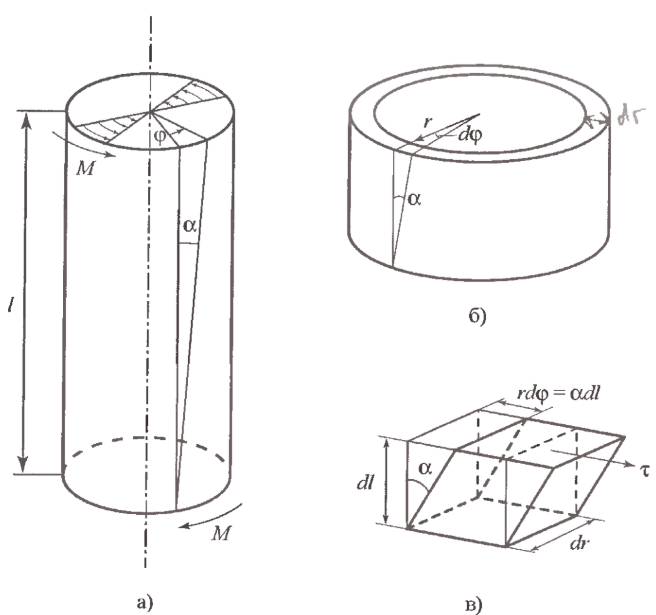
\includegraphics[width=11cm]{1}
\end{center} 

По закону Гука касательное напряжение $\tau$ связано с углом сдвига $\alpha$ линейной зависимостью, в которую входит модуль сдвига $G$:
\[\tau = G \alpha\]

Комбинируя две последние записанные формулы, имеем:
\[\tau = G \alpha = G r \frac{d\varphi}{d l}\]

Касательное напряжение создаёт момент сил относительно оси цилиндра:
\[dM = \tau dS  r = 2 \pi r dr \tau r = 2 \pi G \frac{d\varphi}{d l} r^3 dr\]

Суммарный момент сил, действующий на всём поперечном сечении цилиндра, равен

\[M = \int_M dM = \int_0^{R}2 \pi G \frac{d\varphi}{d l} r^3 dr = \pi G \frac{d\varphi}{d l} \frac{R^4}{2}\]

Так как стержень находится в равновесии, то момент, записанный выше, постоянен, значит постоянно и выражение
\[\frac{d\varphi}{d l} = const \Rightarrow \varphi = const \cdot l \text{ (с учётом граничных условий)}\]

\[M = \frac{\pi G R^4}{2l} \varphi = f \varphi\]

Здесь была введена вспомогательная величина $f$ -- модуль кручения. 

Следует отметить, что полученная формула справедлива только малых значений касательного напряжения.\\


\section{Ход работы}
\subsection{Определение модуля кручения статическим методом}

В этой части эксперимента воспользуемся следующей схемой экспериментальной установки для определения модуля кручения:

Верхний конец вертикально расположенного стержня С жёстко закреплён на стойке, а нижний соединён с диском Д. Момент $M$, закручивающий стержень, создают две навитые на диск и перекинутые через блоки Б нити, к концам которых подвешиваются одинаковые грузы Г. Диск снабжён зеркальцем З. Для определения угла закручивания стержня надо зрительную трубу направить на зеркальце и добиться того, чтобы в неё было чётко видно отражение шкалы, укреплённой на том же штативе, что и труба. Измерение смещения изображения шкалы в трубе позволяет определиь угол закручивания стержня.

Установим зрительную трубу таким образом, чтобы в неё было чётко видно отображение шкалы в зекральце З. 

Измерим расстояние от зеркальца до шкалы Д, определим диаметры стержня и шкива:
\begin{center}
\begin{tabular}{|c|c|c|c|c|c|c|c|c|c|c|}
\hline 
$L$, см & 133,2 & 133,2 & 133,3 & 133,5 & 133,4 & 133,4 & 133,2 & 133,2 & 133,3 & 133,5 \\ 
\hline 
$D$, мм & 5,95 & 5,93 & 5,95 & 5,95 & 5,94 & 5,95 & 5,94 & 5,95 & 5,95 & 5,94 \\ 
\hline 
$R_{\text{Д}}$, см & 10,1 & 10,11 & 10,1 & 10,11 & 10,11 & 10,1 & 10,1 & 10,1 & 10,1 & 10,1 \\ 
\hline 
\end{tabular}
\end{center} 

Рассчитаем средние значения:
\[L = 133,32\text{ см, }D = 5,945\text{ мм, }R = 2,973\text{ мм, }R_{\text{Д}} = 10,103\text{ см}\]

Рассчитаем случайные погрешности:
\[\Delta L_{\text{случ}} = 0,37\text{ см, }\Delta D_{\text{случ}} = \Delta R_{\text{случ}} = 0,002\text{ мм, }\Delta R_{\text{Дслуч}} = 0,02\text{ мм}\]

Систематические погрешности равны $0,1$ см, $0,01$ мм, $0,05$ мм.

\begin{center}
    {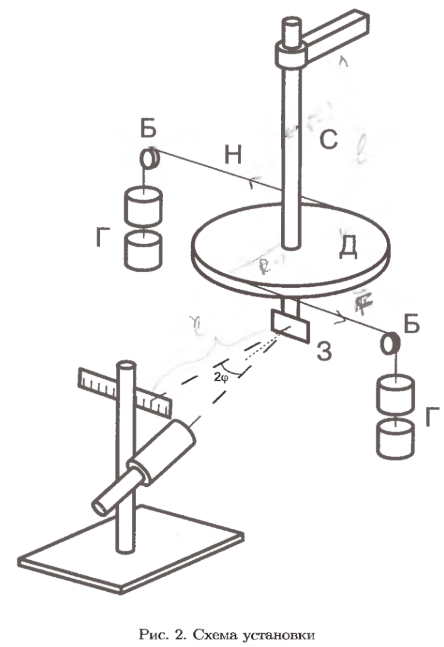
\includegraphics[width=8cm]{2}}
\end{center} 

Рассчитаем погрешности найденных данных:
\[\Delta L = 0,38\text{ см, }\Delta R = 0,01\text{ мм, }\Delta R_{\text{Д}} = 0,054\text{ мм}\]

Увеличивая нагрузку на нитях, снимем зависимость $\varphi (M)$, учитывая, что момент сил равен $M = mgR_{\text{Д}}$. Далее проделываем то же самое, уменьшая нагрузку до нуля. Повторим измерения ещё два раза, занеся всё в таблицы:

\begin{center}
\begin{tabular}{|c|c|c|c|c|c|c|c|}
\hline 
$m$, г & 198 & 396 & 594 & 792 & 594 & 396 & 198 \\ 
\hline 
$x$, см & 9,4 & 17,8 & 26,5 & 34,8 & 27,9 & 17,8 & 9,1 \\ 
\hline 
$x$, см & 9,1 & 17,8 & 26 & 36 & 28 & 17,7 & 9,4 \\ 
\hline 
$x$, см & 9,1 & 17 & 26 & 35 & 27,2 & 17,2 & 9,2 \\ 
\hline 
$x$, см & 9,2 & 17,6 & 25,7 & 34,9 & 28,3 & 17,9 & 9 \\ 
\hline 
\end{tabular} 
\end{center}

\begin{center}
\begin{tabular}{|c|c|c|c|c|c|c|c|}
\hline 
$M$, $\text{Н} \cdot \text{м}$ & 0,1962 & 0,3925 & 0,5887 & 0,785 & 0,5887 & 0,3925 & 0,1962 \\ 
\hline 
$\varphi$& 0,0352 & 0,0664 & 0,0981 & 0,1277 & 0,1031 & 0,0663 & 0,0341 \\ 
\hline 
$\varphi$& 0,0341 & 0,0664 & 0,0963 & 0,1319 & 0,1035 & 0,066 & 0,0352 \\ 
\hline 
$\varphi$& 0,0341 & 0,0634 & 0,0963 & 0,1284 & 0,1007 & 0,0642 & 0,0345 \\ 
\hline 
$\varphi$& 0,0345 & 0,0656 & 0,0952 & 0,128 & 0,1046 & 0,0667 & 0,0337 \\ 
\hline 
\end{tabular} 
\end{center}

Построим график полученной зависимости $\varphi (M)$ для четырёх снятых зависимостей. 

Определим по методу наименьших квадратов модуль кручения и его прогрешность:
\[f = \frac{\langle M  \varphi \rangle}{\langle \varphi^2 \rangle } = \frac{0,0406}{0,00682}\text{ Н} \cdot \text{м} = 5,95\text{ Н} \cdot \text{м}\]
\[\text{ } \Delta f = \sqrt{\frac{1}{N-1} \Big( \frac{\langle M^2 \rangle}{\langle \varphi^2 \rangle} - f^2 \Big)} = \sqrt{\frac{1}{27} \Big( \frac{0,242}{0,0273} - 2,974^2 \Big)} = 0,047\text{ Н} \cdot \text{м}\]

Теперь посчитаем модуль сдвига и его погрешность:
\[G = \frac{2fL}{\pi R^4} = 6,464 \cdot 10^{10}\text{ Н} \cdot \text{м}^{-2}\]
\[\Delta G = G \sqrt{\Big( \frac{\Delta f}{f}\Big) ^2 + \Big(\frac{\Delta L}{L} \Big)^2 + \Big(4\frac{\Delta R}{R} \Big)^2}= 0,102 \cdot 10^{10}\text{ Н} \cdot \text{м}^{-2}\]

\subsection{Определение модуля кручения при помощи кртильных колебаний}

Экспериментальнеая установка (см рис.), используемая в этой части, состоит из длинной вертикально висящей проволоки П, к нижнему концу которой прикреплён горизонтальный металлический стержень С с двумя симметрично расположенными грузами Г. Их положение не стержне можно фиксировать. Верхний конец проволоки зажат в цангу и при помощи специального приспособления может вместе с цангой поворачиваться вокруг вертикальной оси. Таким способом в системе можно возбуждать крутильные колебания. 

Вращение стержня С с закреплёнными на нём грузами Г вокруг вертикальной оси происходит под действием упругого момента, возникающего в проволоке. Оно описывается уравнением
\[I \frac{d^2 \varphi}{d t^2} = -M = -f \varphi\]

Здесь $I$ -- момент инерции стержня с грузами относительно оси вращения, $\varphi$ -- угол поворота стержня от положения равновесия, а $M$ -- момент сил, действующий на стержень. 

\begin{center}
    {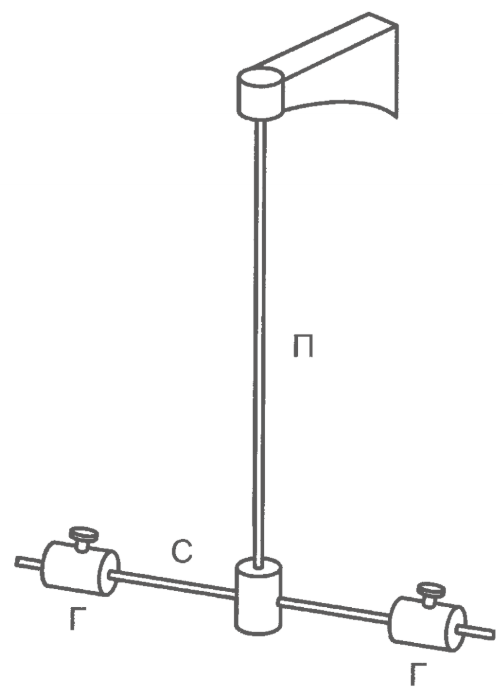
\includegraphics[width=8cm]{3}}
\end{center}

Полученное дифференциальное уравнение имеет решение
\[\varphi = \varphi_0 sin(\omega t + \theta)\]

Здесь начальная фаза $\theta$ и амплитуда колебаний $\varphi_0$ задаются начальными условиями, а $\omega = \sqrt{\frac{f}{I}}$.

Период колебаний равен 
\[T = 2 \pi \sqrt{\frac{I}{f}} \]

Теперь важно понять, что уравнение движения было составлено без учёта диссипативных сил, соответственно было получено решение для незатухающий колебаний. Но в этом ещё надо убедиться: для оценки можно положить, что рассматриваемые колебания действительно незатухающие, если логарифмический декремент затухания меньше, чем $0,1$:
\[\lambda = ln\frac{\varphi (t)}{\varphi (t + T)} = \frac{1}{N} < \frac{1}{10} \Rightarrow N > 10\]

Здесь $N$ -- количество колебаний, за которое амплитуда уменьшается в $e$ раз. Вывод записанной формулы следует из уравнения затухающих колебаний.

Для начала установим диапазон амплитуд, в котором применимы результаты, полученные для незатухающий колебаний, в частности независимость периода колебаний от амплитуды. Для этого укрепим грузы на некотором расстоянии от проволоки и возбудим в системе крутильные колебания. Измерив порядка $10$ периодов колебания для некоторой выбранной амплитуды, находим этот период колебания $T_1$. Теперь находим таким же способом период колебаний $T_2$, где амплитуда колебаний в два раза меньше. Если периоды совпадают, то будем брать амплитуды не больше выбранной, если не совпадают, то берём более мелкую амплитуду и повторяем действия.  

Теперь убедимся в том, что логарифмический декремент затухания больше меньше $1/10$. Зафиксируем начальную амплитуду и посмотрим, как она поменяется спустя $10$ колебаний. Получаем, что амплитуда изменил меньше, чем в 2 раза, значит она тем более изменилась меньше, чем в $e$ раз.

Меняя расстояние от начала оси до грузов $l$, будем измерять период колебаний системы $T$. Каждое имзерение проводим $6$ раз. Запишем все данные в таблицу:

\begin{center}
\begin{tabular}{|c|c|c|c|c|c|c|c|}
\hline 
$l$, см & 4,25 & 5,25 & 6,25 & 7,25 & 8,25 & 9,25 & 11,25 \\ 
\hline 
$T$, с & 2,168 & 2,505 & 2,668 & 2,906 & 3,171 & 3,407 & 3,981 \\ 
\hline 
$T$, с & 2,127 & 2,491 & 2,670 & 2,926 & 3,153 & 3,415 & 3,962 \\ 
\hline 
$T$, с & 2,146 & 2,473 & 2,593 & 2,951 & 3,091 & 3,456 & 4,001 \\ 
\hline 
$T$, с & 2,173 & 2,469 & 2,629 & 2,883 & 3,184 & 3,388 & 3,958 \\ 
\hline 
$T$, с & 2,118 & 2,502 & 2,679 & 2,946 & 3,157 & 3,421 & 3,974 \\ 
\hline 
$T$, с & 2,10 & 2,482 & 2,632 & 2,913 & 3,133 & 3,472 & 3,997 \\ 
\hline 
\end{tabular}
\end{center} 

В данном случае можно провести следующую линеаризацию:
\[T^2 = \frac{4\pi^2 I}{f}\]

Момент инерции из-за больших размеров грузов сильно меняется, поэтому использовать аппроксимацию материальной точки нельзя. Нужно посчитать момент инерции для каждой длины. 

Для начала выведем формулу для момента инерции. Начнём с того, что выведем момент инерции для диска радиуса $R$, находящегося на расстоянии $l$ от рассматриваемой оси:

\[dm = \sigma dS = \sigma 2\pi r dr = \frac{m}{\pi R^2} 2\pi r dr = \frac{2m}{R^2} r dr\]
\[I = \int_{I} (r^2 + l^2) dm = \frac{2m}{R^2}\Big(\int_{0}^{R} r^3 dr + l^2\int_{0}^{R} r dr \Big) = \]
\[= \frac{m}{R^2}\Big(\frac{R^4}{2} + l^2 R^2 \Big) = m\Big(\frac{R^2}{2} + l^2 \Big)\]

Теперь представим, что мы рассматриваем бесконечно тонкий диск толщиной $dl$, значит для него выполняется
\[dI = dm\Big(\frac{R^2}{2} + l^2 \Big) = \frac{m}{L} dl\Big(\frac{R^2}{2} + l^2 \Big) \]
\[I = \frac{m}{L} \int_{l}^{l+L} \Big(\frac{R^2}{2} + l^2 \Big) dl = \frac{m}{L} \Big(\frac{L R^2}{2} + \int_{l}^{l+L} l^2 dl \Big) = \frac{m}{L} \Big(\frac{L R^2}{2} + \frac{(l+L)^3 - l^3}{3} \Big) \]
\[I = \frac{m}{L}\Big(\frac{R^2 L}{2} + \frac{1}{3}\big((l + L)^3 - l^3\big)\big)\]

Для нашей ситуации надо брать в расчёт два груза  ещё нужно учесть, что у системы есть собственный момент инерции, тогда
\[I = \frac{2m}{L}\Big(\frac{R^2 L}{2} + \frac{1}{3}\big((l + L)^3 - l^3\big)\big) +  I_0 = I_1 + I_0\]

Здесь у нас $l$ -- расстояние от оси до цилиндра, $L = 4$ см -- длина самого цилиндрического груза, $R = 2$ см -- радиус цилиндрического груза, а $m = 375$ г -- масса цилиндрического груза, $I_0$ -- момент инерции системы без грузов.

Найдём собственный момент инерции системы. Для этого посчитаем период колебаний системы без грузов:

\begin{center}
\begin{tabular}{|c|c|c|c|c|c|c|c|c|}
\hline 
$T$, с & 1,145 & 1,131 & 1,121 & 1,155 & 1,144 & 1,134 & 1,128 & 1,129 \\ 
\hline 
\end{tabular}
\end{center} 

Найдём среднюю величину $\langle T \rangle = 1,136$ и её погрешность: $\Delta \langle T \rangle = 0,012$ с. Также полезными будут значения $\langle T \rangle^2 = 1,29 \text{ с}^2$ и $\Delta \langle T \rangle^2 = 2 \langle T \rangle \Delta \langle T \rangle  = 0,027 \text{ с}^2$. Для собственного момента инерции имеем:
\[I_0 = \frac{\langle T \rangle^2}{4\pi^2}f\]

Значит формула для периода колебаний выглядит так:
\[T^2 = \frac{4\pi^2 (I_1 + I_0)}{f} = T^2 = \frac{4\pi^2 I_1}{f} + \langle T \rangle^2 \Rightarrow T^2 - \langle T \rangle^2 = \frac{4\pi^2 I_1}{f}\]

Строим таблицу для моментов инерции в зависимости от $l$, попутно считая средние значения для периода колебаний и их погрешности:\\

\begin{center}
\begin{tabular}{|c|c|c|c|c|c|c|c|}
\hline 
$l$, см & 4,25 & 5,25 & 6,25 & 7,25 & 8,25 & 9,25 & 11,25 \\ 
\hline 
$I_1 \cdot 10^{-3}$, $\text{кг} \cdot \text{м}^2$  & 3,179 & 4,192 & 5,355 & 6,667 & 8,130 & 9,742 & 13,417 \\ 
\hline 
$T$, с & 2,139 & 2,487 & 2,645 & 2,92 & 3,148 & 3,427 & 3,979 \\ 
\hline 
$\Delta T$, c & 0,054 & 0,014 & 0,03 & 0,023 & 0,03 & 0,03 & 0,016 \\ 
\hline
$T^2$, $\text{с}^2$ & 4,575 & 6,185 & 6,996 & 8,526 & 9,91 & 11,744 & 15,832 \\ 
\hline 
$\Delta (T^2)$, $\text{с}^2$ & 0,4 & 0,07 & 0,16 & 0,13 & 0,19 & 0,21 & 0,13 \\ 
\hline 
$T^2 - \langle T \rangle^2$, $\text{с}^2$ & 3,285 & 4,985 & 5,676 & 7,236 & 8,620 & 10,454 & 14,542 \\ 
\hline 
$\Delta (T^2 - \langle T \rangle^2)$, $\text{с}^2$ & 0,29 & 0,097 & 0,187 & 0,157 & 0,217 & 0,237 & 0,157 \\ 
\hline 
\end{tabular}
\end{center}   

Сразу считаем значения для линеаризации $T^2$, $l^2$, $(\Delta T)^2 = 2 T \Delta T$. Строим график зависимости $T(l)$ и с помощью метода хи-квадрат считаем, чему равен коэффициент линеаризации и его погрешность:

\[\frac{4\pi^2}{f} = \frac{\langle (T^2 - \langle T \rangle^2) I \rangle^{'}}{\langle I^2 \rangle^{'}} = \frac{\sum_{i = 1}^{7} \frac{(T^2 - \langle T \rangle^2)_i}{(\Delta (T^2 - \langle T \rangle^2))^2} I_i}{\sum_{i = 1}^{7} \frac{I^2_i}{(\Delta (T^2 - \langle T \rangle^2))^2}} = \]
\[= \frac{2,304}{2,150} \cdot 10^{3} \text{ Н}^{-1} \cdot \text{м}^{-1} = 1,072 \cdot 10^3 \text{ Н}^{-1} \cdot \text{м}^{-1}\]
\[f = 3,682 \cdot 10^{-2}\text{ Н} \cdot \text{м}\]

\[\Delta \Big(\frac{4\pi^2}{f}\Big) =  \frac{\Delta f}{f} \frac{4\pi^2}{f} = \sqrt{\frac{1}{6}\Big( \frac{\langle (T^2 - \langle T \rangle^2)^2 \rangle}{\langle I^2 \rangle} - \Big(\frac{4\pi^2}{f}\Big)^2\Big)} = \]
\[= \sqrt{\frac{1}{6}\Big( \frac{73,61}{63,117} \cdot 10^6 - \Big(\frac{4\pi^2}{f}\Big)^2\Big)} \text{ Н}^{-1} \cdot \text{м}^{-1} = 18,28 \text{ Н}^{-1} \cdot \text{м}^{-1}\]

\[\Delta f = 6,27 \cdot 10^{-4}\text{ Н} \cdot \text{м}\]

Теперь измерим длину и диаметр стержня:
\begin{center}
\begin{tabular}{|c|c|c|c|c|c|c|c|c|}
\hline 
$L$, см & 144,1 & 144,1 & 144 & 144,2 & 144 & 144 & 144,2 & 144 \\ 
\hline 
$D$, мм & 1,91 & 1,92 & 1,91 & 1,92 & 1,91 & 1,91 & 1,91 & 1,92  \\ 
\hline 
\end{tabular}
\end{center} 

Значит дли длины и радиуса имеем: $L_0 = 1,44075$ м, $\Delta L_0 = 0,0013$ м, $D = 1,914$ мм, $\Delta D = \sqrt{1,713^2 + 1^2} \text{ мкм} = 1,983 \text{ мкм}$ 

Теперь посчитаем модуль сдвига и его погрешность:
\[G = \frac{2fL_0}{\pi R^4} = 4,026 \cdot 10^{10}\text{ Н} \cdot \text{м}^{-2}\] 
\[\Delta G = G \sqrt{\Big( \frac{\Delta f}{f}\Big) ^2 + \Big(\frac{\Delta L_0}{L_0} \Big)^2 + \Big(4\frac{\Delta R}{R} \Big)^2}= 8,91 \cdot 10^8 \text{ Н} \cdot \text{м}^{-2}\]


\section{Выводы}

В результате эксперимента измерили углы закручивания стержня в зависимости от приложенного момента сил, рассчитали модуль кручения и сдвига при статическом закручивании стержня, определи те же модули для проволоки по измерениям крутильных колебаний подвешенного на ней маятника (динамическим методом). 

Сравним полученные значения модуля кручения с табличными: в первой части значение модуля кручения совпадает со значением модуля кручения стали ($7,9 \cdot 10^{10}\text{ Н} \cdot \text{м}^{-2}$) или железа $7,7 \cdot 10^{10}\text{ Н} \cdot \text{м}^{-2}$ (значение заниженное из-за того, что стержень часто крутили и он стал более гибким), во второй части значение совпадает с модулем кручения латуни ($3,5 \cdot 10^{10}\text{ Н} \cdot \text{м}^{-2}$) или бронзы ($3,3-3,7 \cdot 10^{10}\text{ Н} \cdot \text{м}^{-2}$).



\end{document}